\documentclass[twoside]{book}

% Packages required by doxygen
\usepackage{fixltx2e}
\usepackage{calc}
\usepackage{doxygen}
\usepackage[export]{adjustbox} % also loads graphicx
\usepackage{graphicx}
\usepackage[utf8]{inputenc}
\usepackage{makeidx}
\usepackage{multicol}
\usepackage{multirow}
\PassOptionsToPackage{warn}{textcomp}
\usepackage{textcomp}
\usepackage[nointegrals]{wasysym}
\usepackage[table]{xcolor}

% Font selection
\usepackage[T1]{fontenc}
\usepackage[scaled=.90]{helvet}
\usepackage{courier}
\usepackage{amssymb}
\usepackage{sectsty}
\renewcommand{\familydefault}{\sfdefault}
\allsectionsfont{%
  \fontseries{bc}\selectfont%
  \color{darkgray}%
}
\renewcommand{\DoxyLabelFont}{%
  \fontseries{bc}\selectfont%
  \color{darkgray}%
}
\newcommand{\+}{\discretionary{\mbox{\scriptsize$\hookleftarrow$}}{}{}}

% Page & text layout
\usepackage{geometry}
\geometry{%
  a4paper,%
  top=2.5cm,%
  bottom=2.5cm,%
  left=2.5cm,%
  right=2.5cm%
}
\tolerance=750
\hfuzz=15pt
\hbadness=750
\setlength{\emergencystretch}{15pt}
\setlength{\parindent}{0cm}
\setlength{\parskip}{3ex plus 2ex minus 2ex}
\makeatletter
\renewcommand{\paragraph}{%
  \@startsection{paragraph}{4}{0ex}{-1.0ex}{1.0ex}{%
    \normalfont\normalsize\bfseries\SS@parafont%
  }%
}
\renewcommand{\subparagraph}{%
  \@startsection{subparagraph}{5}{0ex}{-1.0ex}{1.0ex}{%
    \normalfont\normalsize\bfseries\SS@subparafont%
  }%
}
\makeatother

% Headers & footers
\usepackage{fancyhdr}
\pagestyle{fancyplain}
\fancyhead[LE]{\fancyplain{}{\bfseries\thepage}}
\fancyhead[CE]{\fancyplain{}{}}
\fancyhead[RE]{\fancyplain{}{\bfseries\leftmark}}
\fancyhead[LO]{\fancyplain{}{\bfseries\rightmark}}
\fancyhead[CO]{\fancyplain{}{}}
\fancyhead[RO]{\fancyplain{}{\bfseries\thepage}}
\fancyfoot[LE]{\fancyplain{}{}}
\fancyfoot[CE]{\fancyplain{}{}}
\fancyfoot[RE]{\fancyplain{}{\bfseries\scriptsize Generated by Doxygen }}
\fancyfoot[LO]{\fancyplain{}{\bfseries\scriptsize Generated by Doxygen }}
\fancyfoot[CO]{\fancyplain{}{}}
\fancyfoot[RO]{\fancyplain{}{}}
\renewcommand{\footrulewidth}{0.4pt}
\renewcommand{\chaptermark}[1]{%
  \markboth{#1}{}%
}
\renewcommand{\sectionmark}[1]{%
  \markright{\thesection\ #1}%
}

% Indices & bibliography
\usepackage{natbib}
\usepackage[titles]{tocloft}
\setcounter{tocdepth}{3}
\setcounter{secnumdepth}{5}
\makeindex

% Hyperlinks (required, but should be loaded last)
\usepackage{ifpdf}
\ifpdf
  \usepackage[pdftex,pagebackref=true]{hyperref}
\else
  \usepackage[ps2pdf,pagebackref=true]{hyperref}
\fi
\hypersetup{%
  colorlinks=true,%
  linkcolor=blue,%
  citecolor=blue,%
  unicode%
}

% Custom commands
\newcommand{\clearemptydoublepage}{%
  \newpage{\pagestyle{empty}\cleardoublepage}%
}

\usepackage{caption}
\captionsetup{labelsep=space,justification=centering,font={bf},singlelinecheck=off,skip=4pt,position=top}

%===== C O N T E N T S =====

\begin{document}

% Titlepage & ToC
\hypersetup{pageanchor=false,
             bookmarksnumbered=true,
             pdfencoding=unicode
            }
\pagenumbering{alph}
\begin{titlepage}
\vspace*{7cm}
\begin{center}%
{\Large team18 }\\
\vspace*{1cm}
{\large Generated by Doxygen 1.8.13}\\
\end{center}
\end{titlepage}
\clearemptydoublepage
\pagenumbering{roman}
\tableofcontents
\clearemptydoublepage
\pagenumbering{arabic}
\hypersetup{pageanchor=true}

%--- Begin generated contents ---
\chapter{Hierarchical Index}
\section{Class Hierarchy}
This inheritance list is sorted roughly, but not completely, alphabetically\+:\begin{DoxyCompactList}
\item Auth\+Widget\begin{DoxyCompactList}
\item \contentsline{section}{Auth\+Widget}{\pageref{class_auth_widget}}{}
\end{DoxyCompactList}
\item \contentsline{section}{Group}{\pageref{class_group}}{}
\item Registration\+Widget\begin{DoxyCompactList}
\item \contentsline{section}{Registration\+View}{\pageref{class_registration_view}}{}
\end{DoxyCompactList}
\item Session\begin{DoxyCompactList}
\item \contentsline{section}{Session}{\pageref{class_session}}{}
\end{DoxyCompactList}
\item \contentsline{section}{User}{\pageref{class_user}}{}
\item W\+Application\begin{DoxyCompactList}
\item \contentsline{section}{Auth\+Application}{\pageref{class_auth_application}}{}
\end{DoxyCompactList}
\item W\+Container\+Widget\begin{DoxyCompactList}
\item \contentsline{section}{Bridge}{\pageref{class_bridge}}{}
\end{DoxyCompactList}
\item W\+Form\+Model\begin{DoxyCompactList}
\item \contentsline{section}{User\+Details\+Model}{\pageref{class_user_details_model}}{}
\end{DoxyCompactList}
\end{DoxyCompactList}

\chapter{Class Index}
\section{Class List}
Here are the classes, structs, unions and interfaces with brief descriptions\+:\begin{DoxyCompactList}
\item\contentsline{section}{\hyperlink{class_auth_application}{Auth\+Application} }{\pageref{class_auth_application}}{}
\item\contentsline{section}{\hyperlink{class_auth_widget}{Auth\+Widget} }{\pageref{class_auth_widget}}{}
\item\contentsline{section}{\hyperlink{class_bridge}{Bridge} }{\pageref{class_bridge}}{}
\item\contentsline{section}{\hyperlink{class_group}{Group} }{\pageref{class_group}}{}
\item\contentsline{section}{\hyperlink{class_registration_view}{Registration\+View} }{\pageref{class_registration_view}}{}
\item\contentsline{section}{\hyperlink{class_session}{Session} }{\pageref{class_session}}{}
\item\contentsline{section}{\hyperlink{class_user}{User} }{\pageref{class_user}}{}
\item\contentsline{section}{\hyperlink{class_user_details_model}{User\+Details\+Model} }{\pageref{class_user_details_model}}{}
\end{DoxyCompactList}

\chapter{Class Documentation}
\hypertarget{class_auth_application}{}\section{Auth\+Application Class Reference}
\label{class_auth_application}\index{Auth\+Application@{Auth\+Application}}
Inheritance diagram for Auth\+Application\+:\begin{figure}[H]
\begin{center}
\leavevmode
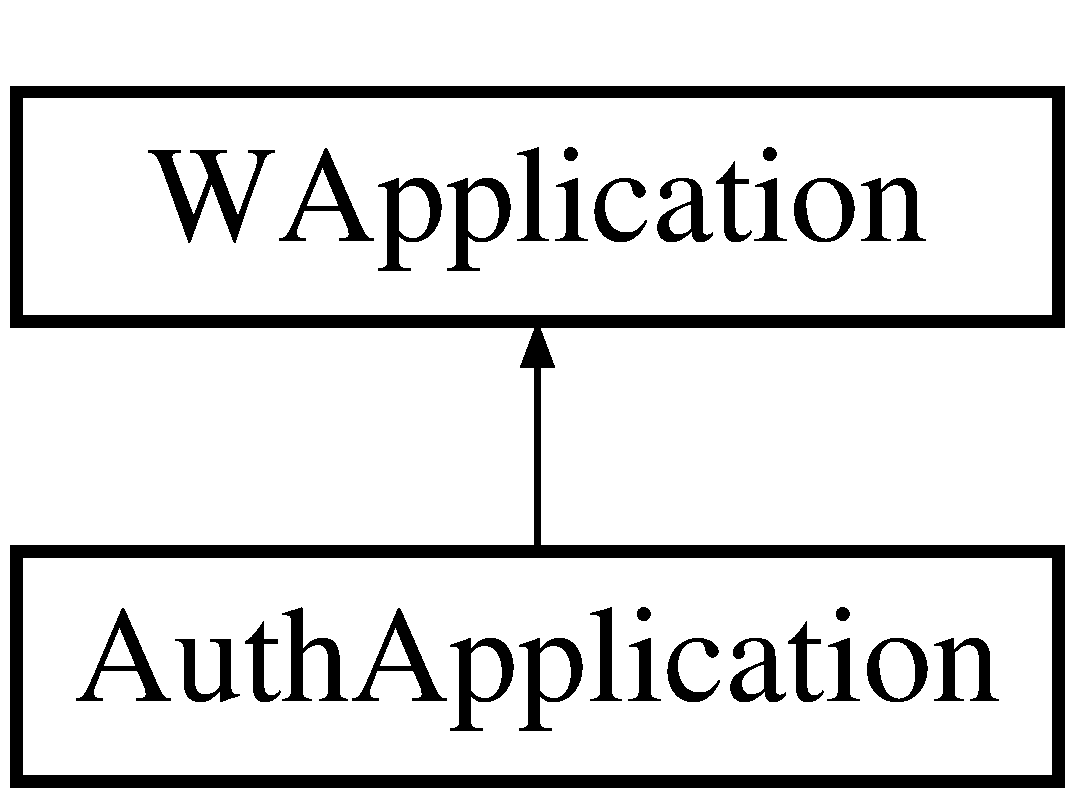
\includegraphics[height=2.000000cm]{class_auth_application}
\end{center}
\end{figure}
\subsection*{Public Member Functions}
\begin{DoxyCompactItemize}
\item 
\mbox{\Hypertarget{class_auth_application_a4d06dfaf02cf7bb4319ce17448d96d2c}\label{class_auth_application_a4d06dfaf02cf7bb4319ce17448d96d2c}} 
{\bfseries Auth\+Application} (const Wt\+::\+W\+Environment \&env)
\item 
\mbox{\Hypertarget{class_auth_application_a48308192a84c5c4b4b14cad505064e4f}\label{class_auth_application_a48308192a84c5c4b4b14cad505064e4f}} 
void {\bfseries to\+Home} ()
\item 
\mbox{\Hypertarget{class_auth_application_a858d1317e8ef7239389dc074e9d2413b}\label{class_auth_application_a858d1317e8ef7239389dc074e9d2413b}} 
void {\bfseries to\+Login} ()
\item 
\mbox{\Hypertarget{class_auth_application_ac88047c5dab3e09322fcf2a7609b0e73}\label{class_auth_application_ac88047c5dab3e09322fcf2a7609b0e73}} 
void {\bfseries to\+Register} ()
\item 
\mbox{\Hypertarget{class_auth_application_a5ef2f6766fa817e850ce6aa7c031d8e2}\label{class_auth_application_a5ef2f6766fa817e850ce6aa7c031d8e2}} 
void {\bfseries auth\+Event} ()
\end{DoxyCompactItemize}


The documentation for this class was generated from the following file\+:\begin{DoxyCompactItemize}
\item 
Auth1.\+cpp\end{DoxyCompactItemize}

\hypertarget{class_auth_widget}{}\section{Auth\+Widget Class Reference}
\label{class_auth_widget}\index{Auth\+Widget@{Auth\+Widget}}
Inheritance diagram for Auth\+Widget\+:\begin{figure}[H]
\begin{center}
\leavevmode
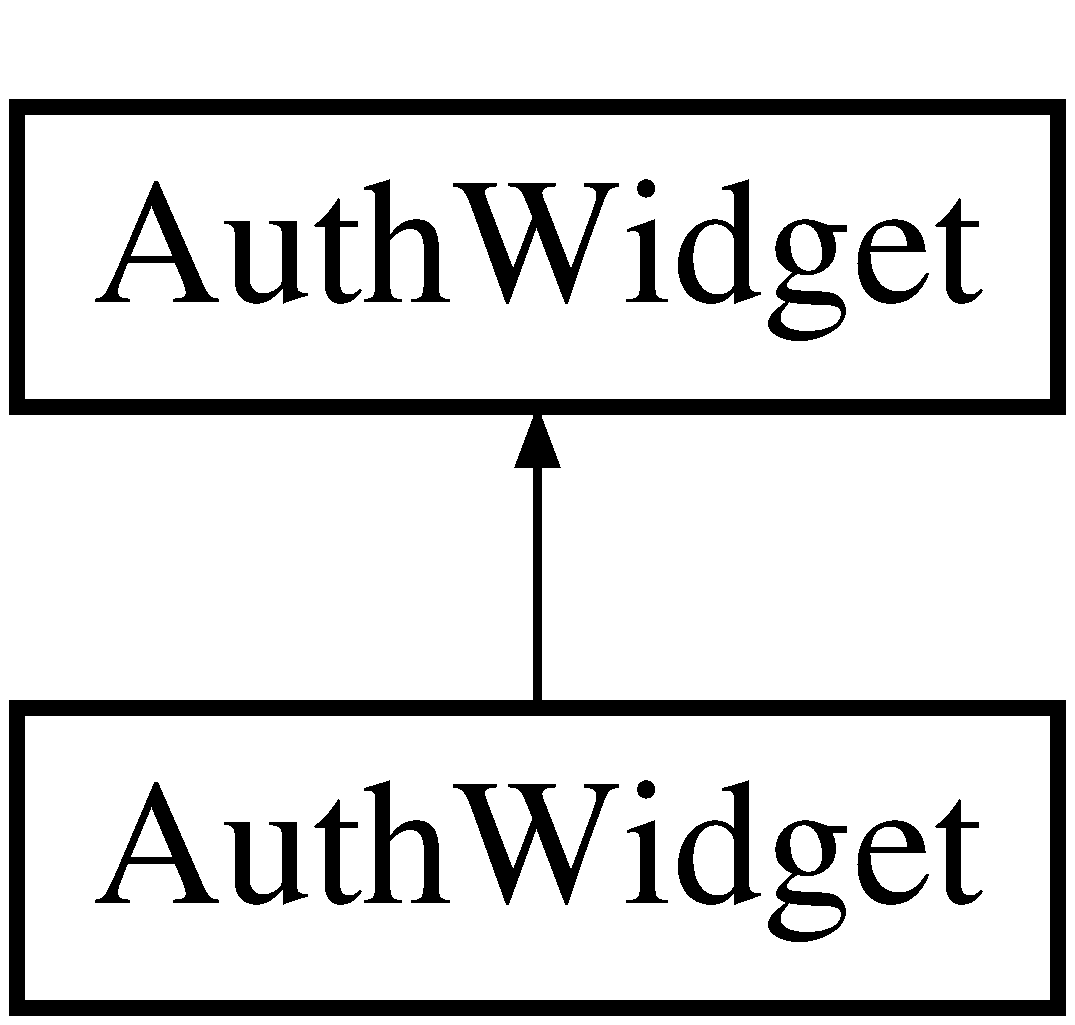
\includegraphics[height=2.000000cm]{class_auth_widget}
\end{center}
\end{figure}
\subsection*{Public Member Functions}
\begin{DoxyCompactItemize}
\item 
\mbox{\Hypertarget{class_auth_widget_a16b0f0ad98e79aa40992cfaa9a00cfde}\label{class_auth_widget_a16b0f0ad98e79aa40992cfaa9a00cfde}} 
{\bfseries Auth\+Widget} (\hyperlink{class_session}{Session} \&session)
\item 
\mbox{\Hypertarget{class_auth_widget_abfa295703272e72a5d57dd736cc9f329}\label{class_auth_widget_abfa295703272e72a5d57dd736cc9f329}} 
virtual Wt\+::\+W\+Widget $\ast$ {\bfseries create\+Registration\+View} (const Wt\+::\+Auth\+::\+Identity \&id)
\end{DoxyCompactItemize}


The documentation for this class was generated from the following files\+:\begin{DoxyCompactItemize}
\item 
Auth\+Widget.\+h\item 
Auth\+Widget.\+cpp\end{DoxyCompactItemize}

\hypertarget{class_bridge}{}\section{Bridge Class Reference}
\label{class_bridge}\index{Bridge@{Bridge}}
Inheritance diagram for Bridge\+:\begin{figure}[H]
\begin{center}
\leavevmode
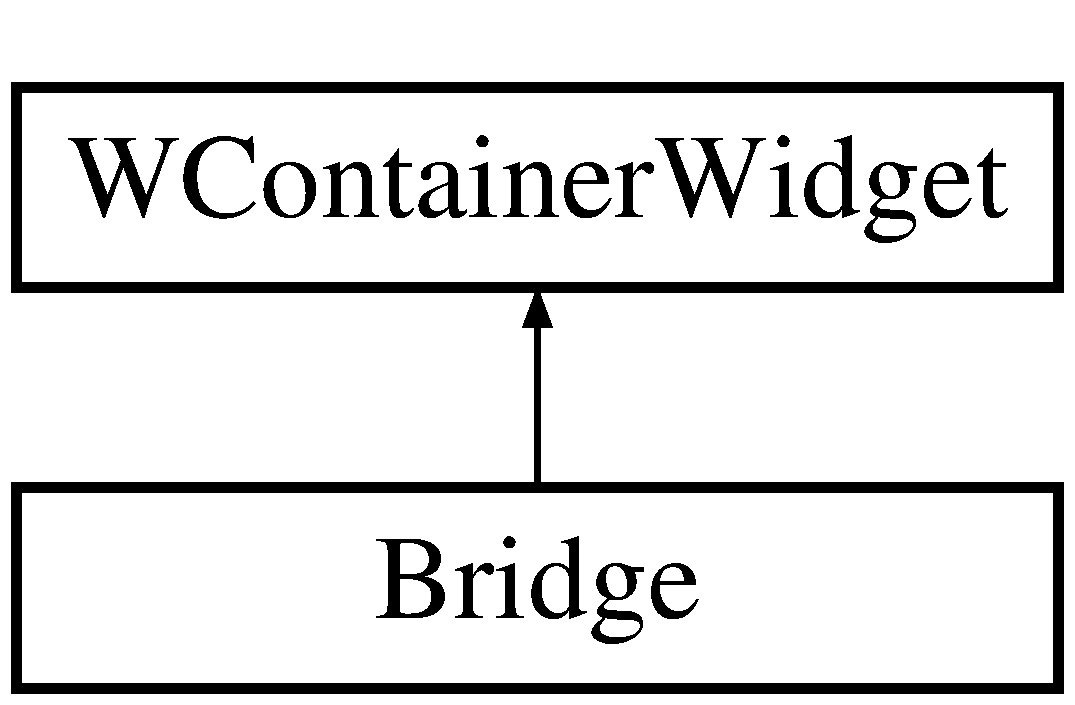
\includegraphics[height=2.000000cm]{class_bridge}
\end{center}
\end{figure}
\subsection*{Public Member Functions}
\begin{DoxyCompactItemize}
\item 
\mbox{\Hypertarget{class_bridge_a01c40750ef65ff1d3e298ba9b6a84365}\label{class_bridge_a01c40750ef65ff1d3e298ba9b6a84365}} 
{\bfseries Bridge} (W\+Container\+Widget $\ast$parent=0)
\item 
\mbox{\Hypertarget{class_bridge_a20b4d278bc879a5c647e106e03fa1cdc}\label{class_bridge_a20b4d278bc879a5c647e106e03fa1cdc}} 
{\footnotesize template$<$class Action $>$ }\\void {\bfseries persist} (Action \&a)
\item 
\mbox{\Hypertarget{class_bridge_a08a06b026240f611629a51655939af28}\label{class_bridge_a08a06b026240f611629a51655939af28}} 
void {\bfseries new\+User\+Connect} (string address, string port, string devicetype, string username, string reference)
\item 
\mbox{\Hypertarget{class_bridge_aed8f97f1934206c5de749598c77c535f}\label{class_bridge_aed8f97f1934206c5de749598c77c535f}} 
void {\bfseries default\+Connect} (string address, string port, string reference)
\item 
\mbox{\Hypertarget{class_bridge_a1378c7a7a02b7048d6d6b25d002fd37c}\label{class_bridge_a1378c7a7a02b7048d6d6b25d002fd37c}} 
void {\bfseries modify\+Bridge} (string address, string port, string username, string reference)
\item 
\mbox{\Hypertarget{class_bridge_ac10faba92bde0ec0f9e5a249a8d50a36}\label{class_bridge_ac10faba92bde0ec0f9e5a249a8d50a36}} 
void {\bfseries test\+Bridge} (string address, string port, string username)
\item 
\mbox{\Hypertarget{class_bridge_afacac6900e4bc45782fe0863817455d8}\label{class_bridge_afacac6900e4bc45782fe0863817455d8}} 
void {\bfseries get\+\_\+all\+Lights} ()
\item 
\mbox{\Hypertarget{class_bridge_a8754c9f194c997a1cfe5ed111ceddef1}\label{class_bridge_a8754c9f194c997a1cfe5ed111ceddef1}} 
void {\bfseries get\+\_\+one\+Light} (string light\+\_\+id)
\item 
\mbox{\Hypertarget{class_bridge_a9c44afd9c931325e73f03ba62b49c2e0}\label{class_bridge_a9c44afd9c931325e73f03ba62b49c2e0}} 
void {\bfseries change\+\_\+light\+Name} (string light\+\_\+id, string light\+\_\+name)
\item 
\mbox{\Hypertarget{class_bridge_a13c3c997050afad67371f3027c63a975}\label{class_bridge_a13c3c997050afad67371f3027c63a975}} 
void {\bfseries change\+\_\+light\+Turn} (string light\+\_\+id, string true\+O\+Rfalse)
\item 
\mbox{\Hypertarget{class_bridge_a9c084f919c36bf11272c3177978f59f0}\label{class_bridge_a9c084f919c36bf11272c3177978f59f0}} 
void {\bfseries change\+\_\+light\+Colour} (string light\+\_\+id, string colour\+Code)
\item 
\mbox{\Hypertarget{class_bridge_a60889f70bfd4cc4f0b63859f2656ca21}\label{class_bridge_a60889f70bfd4cc4f0b63859f2656ca21}} 
void {\bfseries change\+\_\+light\+Brightness} (string light\+\_\+id, string brightness)
\item 
\mbox{\Hypertarget{class_bridge_a30fa03f30ee52a0eb8661b79763b32c5}\label{class_bridge_a30fa03f30ee52a0eb8661b79763b32c5}} 
void {\bfseries set\+\_\+temp\+Add} (string add)
\item 
\mbox{\Hypertarget{class_bridge_ac38732876e444d204e0bf47b36169749}\label{class_bridge_ac38732876e444d204e0bf47b36169749}} 
string {\bfseries get\+\_\+temp\+Add} ()
\item 
\mbox{\Hypertarget{class_bridge_a57fdc9c4f565cdb468b0d8db9ac5ac84}\label{class_bridge_a57fdc9c4f565cdb468b0d8db9ac5ac84}} 
void {\bfseries set\+\_\+temp\+Port} (string port)
\item 
\mbox{\Hypertarget{class_bridge_ae192e205a6e6c50f23b46865cc643668}\label{class_bridge_ae192e205a6e6c50f23b46865cc643668}} 
string {\bfseries get\+\_\+temp\+Port} ()
\item 
\mbox{\Hypertarget{class_bridge_afd4d7c78bb467dc96cf1d4888b972bfa}\label{class_bridge_afd4d7c78bb467dc96cf1d4888b972bfa}} 
void {\bfseries set\+\_\+temp\+User} (string user)
\item 
\mbox{\Hypertarget{class_bridge_ae4fdb6ba396078ec6276e397ad6a05ba}\label{class_bridge_ae4fdb6ba396078ec6276e397ad6a05ba}} 
string {\bfseries get\+\_\+temp\+User} ()
\item 
\mbox{\Hypertarget{class_bridge_a0d8a78cf0597dcdfb346595641704a3d}\label{class_bridge_a0d8a78cf0597dcdfb346595641704a3d}} 
void {\bfseries set\+\_\+temp\+Ref} (string ref)
\item 
\mbox{\Hypertarget{class_bridge_a2bcd54d0d6e8cd86afdec7391233b117}\label{class_bridge_a2bcd54d0d6e8cd86afdec7391233b117}} 
string {\bfseries get\+\_\+temp\+Ref} ()
\item 
\mbox{\Hypertarget{class_bridge_a835d13dc3ba620bef30e92a7dbb0baa4}\label{class_bridge_a835d13dc3ba620bef30e92a7dbb0baa4}} 
void {\bfseries set\+\_\+reference} (string the\+\_\+reference)
\item 
\mbox{\Hypertarget{class_bridge_a25786b8fc161a3b05199269ce89162a9}\label{class_bridge_a25786b8fc161a3b05199269ce89162a9}} 
string {\bfseries get\+\_\+reference} ()
\item 
\mbox{\Hypertarget{class_bridge_a6b34d672f46d2bb2f9bc43d79618eec7}\label{class_bridge_a6b34d672f46d2bb2f9bc43d79618eec7}} 
void {\bfseries set\+\_\+user\+Name} (string the\+\_\+name)
\item 
\mbox{\Hypertarget{class_bridge_a7e92805149031acb4f470957de2622da}\label{class_bridge_a7e92805149031acb4f470957de2622da}} 
string {\bfseries get\+\_\+user\+Name} ()
\item 
\mbox{\Hypertarget{class_bridge_a363f5dff05e0b7c7545c61dbd3dc9d66}\label{class_bridge_a363f5dff05e0b7c7545c61dbd3dc9d66}} 
void {\bfseries set\+\_\+address} (string the\+\_\+address)
\item 
\mbox{\Hypertarget{class_bridge_ac2927ee5c443aec94d12fa318b8b259f}\label{class_bridge_ac2927ee5c443aec94d12fa318b8b259f}} 
string {\bfseries get\+\_\+address} ()
\item 
\mbox{\Hypertarget{class_bridge_afafbafb003d63e36a43d237b184dbd2a}\label{class_bridge_afafbafb003d63e36a43d237b184dbd2a}} 
void {\bfseries set\+\_\+port} (string the\+\_\+port)
\item 
\mbox{\Hypertarget{class_bridge_a48c953016b085bc9c2071ce48bf38a54}\label{class_bridge_a48c953016b085bc9c2071ce48bf38a54}} 
string {\bfseries get\+\_\+port} ()
\item 
\mbox{\Hypertarget{class_bridge_a18ace55fb18a74458da6e29c06a9920b}\label{class_bridge_a18ace55fb18a74458da6e29c06a9920b}} 
void {\bfseries set\+\_\+default\+Response} (string response)
\item 
\mbox{\Hypertarget{class_bridge_aff5c24c0793bee3277764085d26b4b05}\label{class_bridge_aff5c24c0793bee3277764085d26b4b05}} 
string {\bfseries get\+\_\+default\+Response} ()
\item 
\mbox{\Hypertarget{class_bridge_a04e4df5d6d5f5a67a24a141bd4eba69f}\label{class_bridge_a04e4df5d6d5f5a67a24a141bd4eba69f}} 
void {\bfseries set\+\_\+new\+User\+Response} (string response)
\item 
\mbox{\Hypertarget{class_bridge_a3903f77bc9e2f91aa0bdde4d176648f3}\label{class_bridge_a3903f77bc9e2f91aa0bdde4d176648f3}} 
string {\bfseries get\+\_\+new\+User\+Response} ()
\item 
\mbox{\Hypertarget{class_bridge_ab2a198dffad232ed114b76974fc5dab8}\label{class_bridge_ab2a198dffad232ed114b76974fc5dab8}} 
void {\bfseries set\+\_\+modify\+Response} (string response)
\item 
\mbox{\Hypertarget{class_bridge_a7585fb161fa8beb13cd799dab7219e9d}\label{class_bridge_a7585fb161fa8beb13cd799dab7219e9d}} 
string {\bfseries get\+\_\+modify\+Response} ()
\item 
\mbox{\Hypertarget{class_bridge_ac127889bab11771234bca1f979a7a256}\label{class_bridge_ac127889bab11771234bca1f979a7a256}} 
void {\bfseries set\+\_\+\+U\+RL} (string the\+\_\+url)
\item 
\mbox{\Hypertarget{class_bridge_af75ec43258bbe6f7b0a75843c2330537}\label{class_bridge_af75ec43258bbe6f7b0a75843c2330537}} 
string {\bfseries get\+\_\+\+U\+RL} ()
\item 
\mbox{\Hypertarget{class_bridge_a43c11c79e297eca19b1791a9c190b110}\label{class_bridge_a43c11c79e297eca19b1791a9c190b110}} 
void {\bfseries set\+\_\+success} (string flag)
\item 
\mbox{\Hypertarget{class_bridge_a11d8ba5fedcc58a368f912dd604e6841}\label{class_bridge_a11d8ba5fedcc58a368f912dd604e6841}} 
string {\bfseries get\+\_\+success} ()
\item 
\mbox{\Hypertarget{class_bridge_a8d5ccebeec122a6113c034f647ddfff4}\label{class_bridge_a8d5ccebeec122a6113c034f647ddfff4}} 
void {\bfseries set\+\_\+modify\+Success} (string flag)
\item 
\mbox{\Hypertarget{class_bridge_ac55f7ccf6a539f3e1b6a1ba5365b6caa}\label{class_bridge_ac55f7ccf6a539f3e1b6a1ba5365b6caa}} 
string {\bfseries get\+\_\+modify\+Success} ()
\item 
\mbox{\Hypertarget{class_bridge_a2fc01183bf0199ea09c10a14fa408f31}\label{class_bridge_a2fc01183bf0199ea09c10a14fa408f31}} 
void {\bfseries set\+\_\+light\+Success} (string flag)
\item 
\mbox{\Hypertarget{class_bridge_a689b8f5bbebac2d078bb675f386bbe1b}\label{class_bridge_a689b8f5bbebac2d078bb675f386bbe1b}} 
string {\bfseries get\+\_\+light\+Success} ()
\item 
\mbox{\Hypertarget{class_bridge_ad5067ef5a7cc8f6649b7b3ad700605a5}\label{class_bridge_ad5067ef5a7cc8f6649b7b3ad700605a5}} 
void {\bfseries set\+\_\+light\+Set} (set$<$ string $>$ set)
\item 
\mbox{\Hypertarget{class_bridge_a9442a175edbb6098a7595e4eb00dce86}\label{class_bridge_a9442a175edbb6098a7595e4eb00dce86}} 
string {\bfseries get\+\_\+light\+Set} ()
\item 
\mbox{\Hypertarget{class_bridge_a7c1963452e0e7065649b88c5a1f003b9}\label{class_bridge_a7c1963452e0e7065649b88c5a1f003b9}} 
set$<$ string $>$ {\bfseries get\+\_\+test\+Set} ()
\item 
\mbox{\Hypertarget{class_bridge_ad1913b3d194f2aa25fe79a4d8b278246}\label{class_bridge_ad1913b3d194f2aa25fe79a4d8b278246}} 
void {\bfseries set\+\_\+one\+Light\+Content} (string content)
\item 
\mbox{\Hypertarget{class_bridge_a7ff075300df5be136b9ae2ca5ecd60a3}\label{class_bridge_a7ff075300df5be136b9ae2ca5ecd60a3}} 
string {\bfseries get\+\_\+one\+Light\+Content} ()
\item 
\mbox{\Hypertarget{class_bridge_ac721f6969c0903fcdf79762adfcd59f6}\label{class_bridge_ac721f6969c0903fcdf79762adfcd59f6}} 
void {\bfseries set\+\_\+new\+Light\+Name\+Response} (string response)
\item 
\mbox{\Hypertarget{class_bridge_a6d31c903fa7aa40ae84f615723579782}\label{class_bridge_a6d31c903fa7aa40ae84f615723579782}} 
string {\bfseries get\+\_\+new\+Light\+Name\+Response} ()
\item 
\mbox{\Hypertarget{class_bridge_a9b55f1e2310798152a1486ceb5b196fc}\label{class_bridge_a9b55f1e2310798152a1486ceb5b196fc}} 
void {\bfseries set\+\_\+new\+Light\+Turn\+Response} (string response)
\item 
\mbox{\Hypertarget{class_bridge_ab59c2c1e9e7224d86ba571f5f81400bf}\label{class_bridge_ab59c2c1e9e7224d86ba571f5f81400bf}} 
string {\bfseries get\+\_\+new\+Light\+Turn\+Response} ()
\item 
\mbox{\Hypertarget{class_bridge_a74dc60e7b3dde4fbbb7af15abe1b0298}\label{class_bridge_a74dc60e7b3dde4fbbb7af15abe1b0298}} 
void {\bfseries set\+\_\+new\+Light\+Colour\+Response} (string response)
\item 
\mbox{\Hypertarget{class_bridge_a48611c8d3c7c0ffcf039eb8089a56f8a}\label{class_bridge_a48611c8d3c7c0ffcf039eb8089a56f8a}} 
string {\bfseries get\+\_\+new\+Light\+Colour\+Response} ()
\item 
\mbox{\Hypertarget{class_bridge_a05222e48ee699274d1340cb811e5977b}\label{class_bridge_a05222e48ee699274d1340cb811e5977b}} 
void {\bfseries set\+\_\+new\+Light\+Brightness\+Response} (string response)
\item 
\mbox{\Hypertarget{class_bridge_a6d2acd39d2dd29ce4bf4f44fe0a6827d}\label{class_bridge_a6d2acd39d2dd29ce4bf4f44fe0a6827d}} 
string {\bfseries get\+\_\+new\+Light\+Brightness\+Response} ()
\end{DoxyCompactItemize}
\subsection*{Public Attributes}
\begin{DoxyCompactItemize}
\item 
\mbox{\Hypertarget{class_bridge_a2315fd734cffa681760940878d3a8e28}\label{class_bridge_a2315fd734cffa681760940878d3a8e28}} 
bool {\bfseries empty\+Obj}
\item 
\mbox{\Hypertarget{class_bridge_ab3fb62c54a0e927030ff4bed1d9478f5}\label{class_bridge_ab3fb62c54a0e927030ff4bed1d9478f5}} 
Json\+::\+Object {\bfseries bridge\+Data}
\item 
\mbox{\Hypertarget{class_bridge_a7aa11901eca1f0af1901a12c81a0b39f}\label{class_bridge_a7aa11901eca1f0af1901a12c81a0b39f}} 
dbo\+::ptr$<$ \hyperlink{class_user}{User} $>$ {\bfseries user}
\end{DoxyCompactItemize}


The documentation for this class was generated from the following files\+:\begin{DoxyCompactItemize}
\item 
Bridge.\+h\item 
Bridge.\+cpp\end{DoxyCompactItemize}

\hypertarget{class_group}{}\section{Group Class Reference}
\label{class_group}\index{Group@{Group}}
\subsection*{Public Member Functions}
\begin{DoxyCompactItemize}
\item 
\mbox{\Hypertarget{class_group_a8723f9bcec8241762d7cfba60fdb5324}\label{class_group_a8723f9bcec8241762d7cfba60fdb5324}} 
void {\bfseries get\+Groups} ()
\item 
\mbox{\Hypertarget{class_group_a78d045341cd63ec0b40970bcc5aa3135}\label{class_group_a78d045341cd63ec0b40970bcc5aa3135}} 
int {\bfseries change\+State} (string group\+Id, string on, string bri, string hue, string sat)
\item 
\mbox{\Hypertarget{class_group_a964bd1f0b83337adbd57ab59f6d74f05}\label{class_group_a964bd1f0b83337adbd57ab59f6d74f05}} 
int {\bfseries set\+Group\+Lights} (string group\+Id, string new\+Lights)
\item 
\mbox{\Hypertarget{class_group_aaeb261e5fd93ebcb640b0bc0d3f9c24c}\label{class_group_aaeb261e5fd93ebcb640b0bc0d3f9c24c}} 
int {\bfseries delete\+Group} (string group\+Id)
\item 
\mbox{\Hypertarget{class_group_af153150353fe6dc3690b75c9a6748528}\label{class_group_af153150353fe6dc3690b75c9a6748528}} 
string {\bfseries get\+State} (string group\+Id)
\item 
\mbox{\Hypertarget{class_group_a6a405fc932a054819e8ae67cbec1537a}\label{class_group_a6a405fc932a054819e8ae67cbec1537a}} 
string {\bfseries get\+Group\+State} ()
\item 
\mbox{\Hypertarget{class_group_a978fe700d69f55e4d433624c4f517457}\label{class_group_a978fe700d69f55e4d433624c4f517457}} 
string {\bfseries get\+Group\+Id\+List} ()
\item 
\mbox{\Hypertarget{class_group_ad61105ec0d0d5a6322b4ba3026a011b3}\label{class_group_ad61105ec0d0d5a6322b4ba3026a011b3}} 
void {\bfseries make\+Group} (string username, string address, string port, string name, string lights)
\item 
\mbox{\Hypertarget{class_group_aaf710c70c017172ea0b56eeecd33d8ec}\label{class_group_aaf710c70c017172ea0b56eeecd33d8ec}} 
const string \& {\bfseries get\+Port} () const
\item 
\mbox{\Hypertarget{class_group_a29c3300630cfbeb89f7a009bd79e9fb9}\label{class_group_a29c3300630cfbeb89f7a009bd79e9fb9}} 
void {\bfseries set\+Port} (const string \&port)
\item 
\mbox{\Hypertarget{class_group_af91b2d26c80bacb79d6fb33e3fe122df}\label{class_group_af91b2d26c80bacb79d6fb33e3fe122df}} 
const string \& {\bfseries get\+Id} () const
\item 
\mbox{\Hypertarget{class_group_a808a6bdb7e099f6c094b34c060eb4fa5}\label{class_group_a808a6bdb7e099f6c094b34c060eb4fa5}} 
void {\bfseries set\+Id} (const string \&id)
\item 
\mbox{\Hypertarget{class_group_aefcfc39a695835631fbb721b184c45bd}\label{class_group_aefcfc39a695835631fbb721b184c45bd}} 
const string \& {\bfseries get\+Name} () const
\item 
\mbox{\Hypertarget{class_group_aa2869e9491a1977088ebbe5a4755dcff}\label{class_group_aa2869e9491a1977088ebbe5a4755dcff}} 
void {\bfseries set\+Name} (const string \&name)
\item 
\mbox{\Hypertarget{class_group_ad4512e295ca4917dade40fc014f9956d}\label{class_group_ad4512e295ca4917dade40fc014f9956d}} 
const string \& {\bfseries get\+Light\+List} () const
\item 
\mbox{\Hypertarget{class_group_aa4889c12bc13e9af2df8233709d523f5}\label{class_group_aa4889c12bc13e9af2df8233709d523f5}} 
void {\bfseries set\+Light\+List} (const string \&light\+List)
\item 
\mbox{\Hypertarget{class_group_a4531f0b1a6cfbe5a3f21e9b49fa9f9f9}\label{class_group_a4531f0b1a6cfbe5a3f21e9b49fa9f9f9}} 
const string \& {\bfseries get\+Username} () const
\item 
\mbox{\Hypertarget{class_group_a7e5eb3f7c92f6afae7a8df75aaa66a68}\label{class_group_a7e5eb3f7c92f6afae7a8df75aaa66a68}} 
void {\bfseries set\+Username} (const string \&username)
\item 
\mbox{\Hypertarget{class_group_ad2f128f7df10f6a13c3dcd361833f145}\label{class_group_ad2f128f7df10f6a13c3dcd361833f145}} 
const string \& {\bfseries get\+Address} () const
\item 
\mbox{\Hypertarget{class_group_ad98b1ef81a6397b52275b5fb7760497c}\label{class_group_ad98b1ef81a6397b52275b5fb7760497c}} 
void {\bfseries set\+Address} (const string \&address)
\item 
\mbox{\Hypertarget{class_group_a039fcd687c3ecb5990b0aed632e78270}\label{class_group_a039fcd687c3ecb5990b0aed632e78270}} 
void {\bfseries set\+Group\+State} (const string \&group\+State)
\item 
\mbox{\Hypertarget{class_group_a8465ae4477e9ec7d26460ee1b5b81e38}\label{class_group_a8465ae4477e9ec7d26460ee1b5b81e38}} 
void {\bfseries set\+Group\+Id\+List} (const string \&group\+Id\+List)
\item 
\mbox{\Hypertarget{class_group_a830acdb0bf78392b36385f3f46b9b03c}\label{class_group_a830acdb0bf78392b36385f3f46b9b03c}} 
string {\bfseries get\+All\+State} (string group\+Id)
\end{DoxyCompactItemize}


The documentation for this class was generated from the following files\+:\begin{DoxyCompactItemize}
\item 
Group.\+h\item 
Group.\+cpp\end{DoxyCompactItemize}

\hypertarget{class_registration_view}{}\section{Registration\+View Class Reference}
\label{class_registration_view}\index{Registration\+View@{Registration\+View}}
Inheritance diagram for Registration\+View\+:\begin{figure}[H]
\begin{center}
\leavevmode
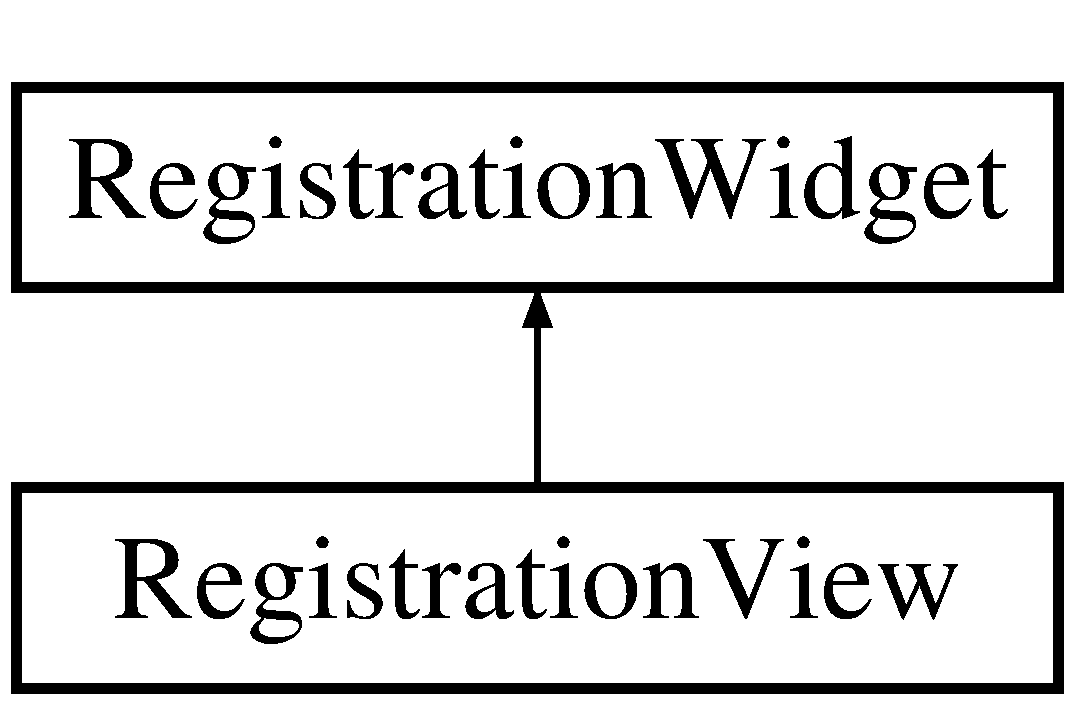
\includegraphics[height=2.000000cm]{class_registration_view}
\end{center}
\end{figure}
\subsection*{Public Member Functions}
\begin{DoxyCompactItemize}
\item 
\mbox{\Hypertarget{class_registration_view_a3848c621b2e4176060293f6f80c16fa7}\label{class_registration_view_a3848c621b2e4176060293f6f80c16fa7}} 
{\bfseries Registration\+View} (\hyperlink{class_session}{Session} \&session, Wt\+::\+Auth\+::\+Auth\+Widget $\ast$auth\+Widget=0)
\item 
\mbox{\Hypertarget{class_registration_view_ae2a0695f816ba4d0f9845b5da6539b34}\label{class_registration_view_ae2a0695f816ba4d0f9845b5da6539b34}} 
virtual Wt\+::\+W\+Widget $\ast$ {\bfseries create\+Form\+Widget} (Wt\+::\+W\+Form\+Model\+::\+Field field)
\end{DoxyCompactItemize}
\subsection*{Protected Member Functions}
\begin{DoxyCompactItemize}
\item 
\mbox{\Hypertarget{class_registration_view_abff4da7c898c36d81a8af6718840d27e}\label{class_registration_view_abff4da7c898c36d81a8af6718840d27e}} 
virtual bool {\bfseries validate} ()
\item 
\mbox{\Hypertarget{class_registration_view_a2e048b6c3103bedacd90a33f6664512b}\label{class_registration_view_a2e048b6c3103bedacd90a33f6664512b}} 
virtual void {\bfseries register\+User\+Details} (Wt\+::\+Auth\+::\+User \&user)
\end{DoxyCompactItemize}


The documentation for this class was generated from the following files\+:\begin{DoxyCompactItemize}
\item 
Registration\+View.\+h\item 
Registration\+View.\+cpp\end{DoxyCompactItemize}

\hypertarget{class_session}{}\section{Session Class Reference}
\label{class_session}\index{Session@{Session}}
Inheritance diagram for Session\+:\begin{figure}[H]
\begin{center}
\leavevmode
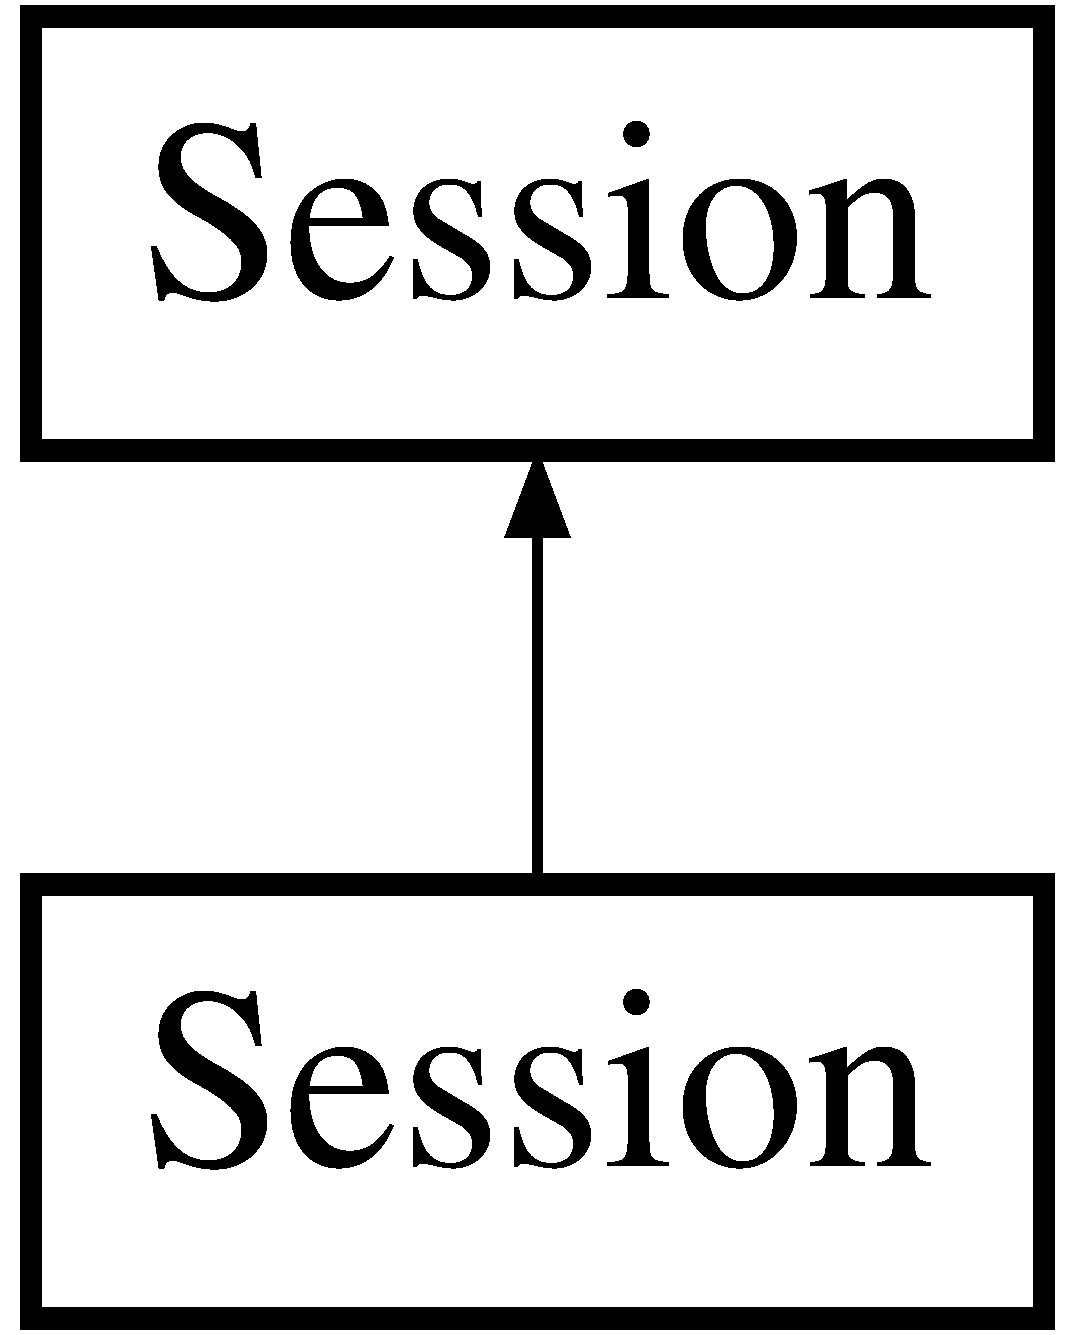
\includegraphics[height=2.000000cm]{class_session}
\end{center}
\end{figure}
\subsection*{Public Member Functions}
\begin{DoxyCompactItemize}
\item 
\mbox{\Hypertarget{class_session_ac5d36ef843286bb362c15d3f465f6b28}\label{class_session_ac5d36ef843286bb362c15d3f465f6b28}} 
{\bfseries Session} (const std\+::string \&sqlite\+Db)
\item 
\mbox{\Hypertarget{class_session_a99e27734249e27c4e916312d09110b4d}\label{class_session_a99e27734249e27c4e916312d09110b4d}} 
dbo\+::ptr$<$ \hyperlink{class_user}{User} $>$ {\bfseries user} () const
\item 
\mbox{\Hypertarget{class_session_a5fa026d211daf8ebed692638dc5f6e96}\label{class_session_a5fa026d211daf8ebed692638dc5f6e96}} 
Wt\+::\+Auth\+::\+Abstract\+User\+Database \& {\bfseries users} ()
\item 
\mbox{\Hypertarget{class_session_ac9b69619756936d8f27bc6702c334b1f}\label{class_session_ac9b69619756936d8f27bc6702c334b1f}} 
Wt\+::\+Auth\+::\+Login \& {\bfseries login} ()
\item 
\mbox{\Hypertarget{class_session_af4b107688e55ec0614d8181688c7dee7}\label{class_session_af4b107688e55ec0614d8181688c7dee7}} 
Wt\+::\+Dbo\+::ptr$<$ \hyperlink{class_user}{User} $>$ {\bfseries user} (const Wt\+::\+Auth\+::\+User \&auth\+User)
\end{DoxyCompactItemize}
\subsection*{Static Public Member Functions}
\begin{DoxyCompactItemize}
\item 
\mbox{\Hypertarget{class_session_a02ee7e0bfcaf6470f35661ec30b8cf8b}\label{class_session_a02ee7e0bfcaf6470f35661ec30b8cf8b}} 
static void {\bfseries configure\+Auth} ()
\item 
\mbox{\Hypertarget{class_session_ab88e346fdd2ca6c3652f612555babf49}\label{class_session_ab88e346fdd2ca6c3652f612555babf49}} 
static const Wt\+::\+Auth\+::\+Auth\+Service \& {\bfseries auth} ()
\item 
\mbox{\Hypertarget{class_session_a4eede16df1d6ca2fe229db43783c8398}\label{class_session_a4eede16df1d6ca2fe229db43783c8398}} 
static const Wt\+::\+Auth\+::\+Password\+Service \& {\bfseries password\+Auth} ()
\item 
\mbox{\Hypertarget{class_session_a1377ccd4db82206d247901fa522bfd8a}\label{class_session_a1377ccd4db82206d247901fa522bfd8a}} 
static const std\+::vector$<$ const Wt\+::\+Auth\+::\+O\+Auth\+Service $\ast$ $>$ \& {\bfseries o\+Auth} ()
\end{DoxyCompactItemize}


The documentation for this class was generated from the following files\+:\begin{DoxyCompactItemize}
\item 
Session.\+h\item 
Session.\+cpp\end{DoxyCompactItemize}

\hypertarget{class_user}{}\section{User Class Reference}
\label{class_user}\index{User@{User}}
\subsection*{Public Member Functions}
\begin{DoxyCompactItemize}
\item 
\mbox{\Hypertarget{class_user_a8169cdbd61e0728531444d666bff1796}\label{class_user_a8169cdbd61e0728531444d666bff1796}} 
void {\bfseries set\+F\+Name} (const std\+::string \&f\+Name)
\item 
\mbox{\Hypertarget{class_user_aeab996acd54819bf0b193349ebe2abc1}\label{class_user_aeab996acd54819bf0b193349ebe2abc1}} 
void {\bfseries set\+L\+Name} (const std\+::string \&l\+Name)
\item 
\mbox{\Hypertarget{class_user_a54095a0a346bc98e20ddd8a5e9b9db20}\label{class_user_a54095a0a346bc98e20ddd8a5e9b9db20}} 
const std\+::string \& {\bfseries get\+F\+Name} () const
\item 
\mbox{\Hypertarget{class_user_a05aebfe0cdbaef0fd0879b28acf36c47}\label{class_user_a05aebfe0cdbaef0fd0879b28acf36c47}} 
const std\+::string \& {\bfseries get\+L\+Name} () const
\item 
\mbox{\Hypertarget{class_user_abe05604556a014f0588aa1f0bcbe3ea8}\label{class_user_abe05604556a014f0588aa1f0bcbe3ea8}} 
const Wt\+::\+Dbo\+::weak\+\_\+ptr$<$ Auth\+Info $>$ \& {\bfseries get\+Auth\+Info} () const
\item 
\mbox{\Hypertarget{class_user_af36fc7ba3c6d8100c0c1c6b383db669a}\label{class_user_af36fc7ba3c6d8100c0c1c6b383db669a}} 
void {\bfseries set\+Auth\+Info} (const Wt\+::\+Dbo\+::weak\+\_\+ptr$<$ Auth\+Info $>$ \&auth\+Info)
\item 
\mbox{\Hypertarget{class_user_a626b516f8e54e0b98c4b20c488de01b8}\label{class_user_a626b516f8e54e0b98c4b20c488de01b8}} 
{\footnotesize template$<$class Action $>$ }\\void {\bfseries persist} (Action \&a)
\item 
\mbox{\Hypertarget{class_user_a0a6fedbf62e9966d9aced7e74dc846ed}\label{class_user_a0a6fedbf62e9966d9aced7e74dc846ed}} 
const string \& {\bfseries get\+Bridge\+Ip} () const
\item 
\mbox{\Hypertarget{class_user_ae80a586ed5c3df0731011bab08199624}\label{class_user_ae80a586ed5c3df0731011bab08199624}} 
void {\bfseries set\+Bridge\+Ip} (const string \&bridge\+Ip)
\item 
\mbox{\Hypertarget{class_user_aeb37fd95e4fe0a4514a3ac5f92f71c90}\label{class_user_aeb37fd95e4fe0a4514a3ac5f92f71c90}} 
const string \& {\bfseries get\+Bridge\+Port} () const
\item 
\mbox{\Hypertarget{class_user_a1367679fc11638d1e767974e2316e88e}\label{class_user_a1367679fc11638d1e767974e2316e88e}} 
void {\bfseries set\+Bridge\+Port} (const string \&bridge\+Port)
\end{DoxyCompactItemize}


The documentation for this class was generated from the following files\+:\begin{DoxyCompactItemize}
\item 
User.\+h\item 
User.\+cpp\end{DoxyCompactItemize}

\hypertarget{class_user_details_model}{}\section{User\+Details\+Model Class Reference}
\label{class_user_details_model}\index{User\+Details\+Model@{User\+Details\+Model}}
Inheritance diagram for User\+Details\+Model\+:\begin{figure}[H]
\begin{center}
\leavevmode
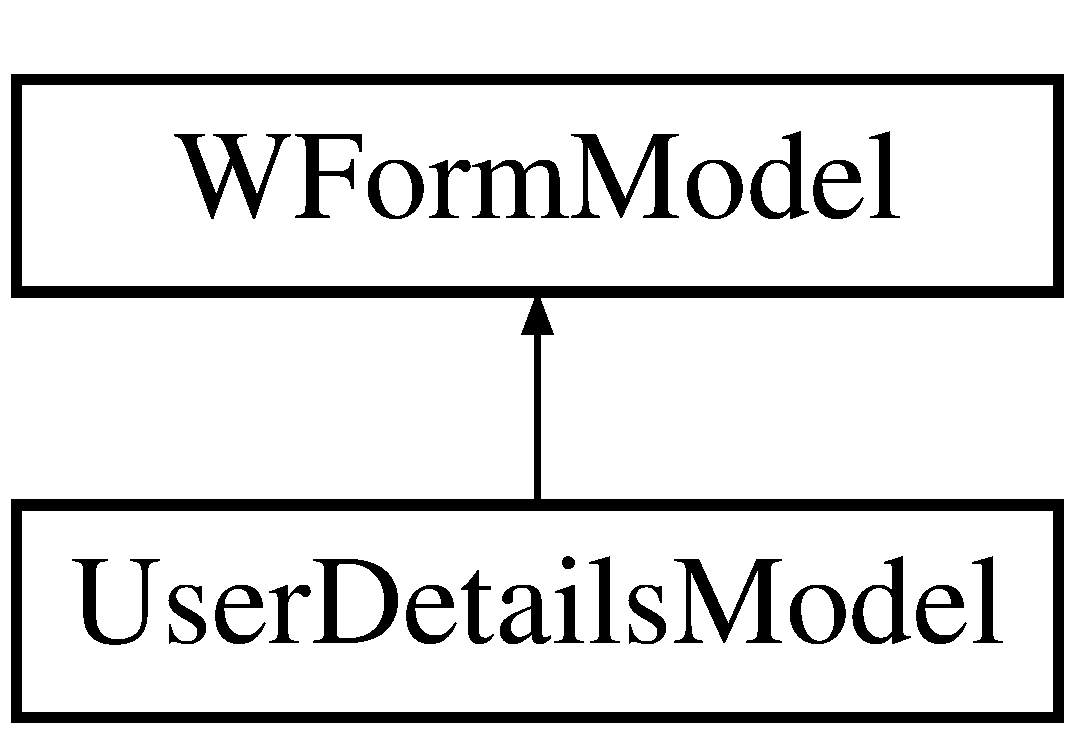
\includegraphics[height=2.000000cm]{class_user_details_model}
\end{center}
\end{figure}
\subsection*{Public Member Functions}
\begin{DoxyCompactItemize}
\item 
\mbox{\Hypertarget{class_user_details_model_aac16af78a18e4a99a6666d85914af5d5}\label{class_user_details_model_aac16af78a18e4a99a6666d85914af5d5}} 
{\bfseries User\+Details\+Model} (\hyperlink{class_session}{Session} \&session, Wt\+::\+W\+Object $\ast$parent=0)
\item 
\mbox{\Hypertarget{class_user_details_model_a0216d9fc37c8528a5fd49756529d4f57}\label{class_user_details_model_a0216d9fc37c8528a5fd49756529d4f57}} 
void {\bfseries save} (const Wt\+::\+Auth\+::\+User \&user)
\end{DoxyCompactItemize}
\subsection*{Static Public Attributes}
\begin{DoxyCompactItemize}
\item 
\mbox{\Hypertarget{class_user_details_model_a0dca416943dc93ce8e1471b7aaeb93ba}\label{class_user_details_model_a0dca416943dc93ce8e1471b7aaeb93ba}} 
static const Field {\bfseries f\+Name\+Field} = \char`\"{}f\+Name\char`\"{}
\item 
\mbox{\Hypertarget{class_user_details_model_af0643d8f4b662e2d05ea142835a15a19}\label{class_user_details_model_af0643d8f4b662e2d05ea142835a15a19}} 
static const Field {\bfseries l\+Name\+Field} = \char`\"{}l\+Name\char`\"{}
\end{DoxyCompactItemize}


The documentation for this class was generated from the following files\+:\begin{DoxyCompactItemize}
\item 
User\+Details\+Model.\+h\item 
User\+Details\+Model.\+cpp\end{DoxyCompactItemize}

%--- End generated contents ---

% Index
\backmatter
\newpage
\phantomsection
\clearemptydoublepage
\addcontentsline{toc}{chapter}{Index}
\printindex

\end{document}
